\chapter{DX-052 NO\_COLOR Is Not a Capability}\label{record-147}

\noindent{\footnotesize\color{BookMuted}\path{docs/design/DX-052-no-color-is-not-a-capability.md}\par}\smallskip

\begin{RecordMeta}
title: DX-052 NO_COLOR Is Not a Capability
legend: DX
lane: release
priority: high
github_issue: 518
status: landed
keywords:
  - no-color
  - output-mode
  - detection
  - theme
  - accessors
  - fallback
  - extend-theme
  - breaking-change
  - v8.0.0

\end{RecordMeta}

\section{Problem}\label{record-147-problem}

Three defects found by an application (\texttt{m\allowbreak{}u\allowbreak{}n\allowbreak{}i\allowbreak{}m\allowbreak{}e\allowbreak{}n\allowbreak{}t}) that had to work around all three locally before it could ship a readable palette. Each one is a case of bijou answering a question the caller did not ask.

\subsection{\texorpdfstring{1. \texttt{N\allowbreak{}O\allowbreak{}\_\allowbreak{}C\allowbreak{}O\allowbreak{}L\allowbreak{}O\allowbreak{}R} takes the whole TUI down, not just the colour}{1.  takes the whole TUI down, not just the colour}}\label{record-147-no_color-takes-the-whole-tui-down-not-just-the-colour}

\texttt{d\allowbreak{}e\allowbreak{}t\allowbreak{}e\allowbreak{}c\allowbreak{}t\allowbreak{}O\allowbreak{}u\allowbreak{}t\allowbreak{}p\allowbreak{}u\allowbreak{}t\allowbreak{}M\allowbreak{}o\allowbreak{}d\allowbreak{}e} (\texttt{p\allowbreak{}a\allowbreak{}c\allowbreak{}k\allowbreak{}a\allowbreak{}g\allowbreak{}e\allowbreak{}s\allowbreak{}/\allowbreak{}b\allowbreak{}i\allowbreak{}j\allowbreak{}o\allowbreak{}u\allowbreak{}/\allowbreak{}s\allowbreak{}r\allowbreak{}c\allowbreak{}/\allowbreak{}c\allowbreak{}o\allowbreak{}r\allowbreak{}e\allowbreak{}/\allowbreak{}d\allowbreak{}e\allowbreak{}t\allowbreak{}e\allowbreak{}c\allowbreak{}t\allowbreak{}/\allowbreak{}t\allowbreak{}t\allowbreak{}y\allowbreak{}.\allowbreak{}t\allowbreak{}s}) resolves in this order:

% Presentation of original arrow notation. See flow-manifest.json.
\begin{center}
\begin{tikzpicture}[book flow node/.style={draw=BookHeading,line width=.65pt,fill=BookPanel,rounded corners=1.5pt,align=center,inner sep=5pt,minimum height=10mm,font=\fontsize{9}{11}\selectfont,execute at begin node={\hyphenpenalty=10000\exhyphenpenalty=10000}},book flow edge/.style={-{Latex[length=2mm]},draw=BookHeading,line width=.7pt}]
\node[book flow node,text width=48mm] (n0) at (-3,0) {BIJOU\_\allowbreak{}ACCESSIBLE=1};
\node[book flow node,text width=48mm] (n1) at (3,0) {'accessible'};
\node[book flow node,text width=48mm] (n2) at (-3,-2) {NO\_\allowbreak{}COLOR /\allowbreak{} TERM=dumb};
\node[book flow node,text width=48mm] (n3) at (3,-2) {'pipe'};
\node[book flow node,text width=48mm] (n4) at (-3,-4) {!stdout.\allowbreak{}is\allowbreak{}TTY};
\node[book flow node,text width=48mm] (n5) at (3,-4) {'pipe'};
\node[book flow node,text width=48mm] (n6) at (-3,-6) {CI};
\node[book flow node,text width=48mm] (n7) at (3,-6) {'static'};
\node[book flow node,text width=48mm] (n8) at (-3,-8) {stdout.\allowbreak{}is\allowbreak{}TTY};
\node[book flow node,text width=48mm] (n9) at (3,-8) {'interactive'};
\draw[book flow edge] (n0) -- (n1);
\draw[book flow edge] (n2) -- (n3);
\draw[book flow edge] (n4) -- (n5);
\draw[book flow edge] (n6) -- (n7);
\draw[book flow edge] (n8) -- (n9);
\end{tikzpicture}
\end{center}


The second line conflates two unrelated requests. \href{https://no-color.org}{no-color.org} defines \texttt{N\allowbreak{}O\allowbreak{}\_\allowbreak{}C\allowbreak{}O\allowbreak{}L\allowbreak{}O\allowbreak{}R} as a statement about \textbf{colour}: ``when present, regardless of its value, prevents the addition of ANSI color''. It says nothing about cursor addressing, alternate screens, or interactivity. bijou reads it as a statement about \textbf{capability}, so a user who exports \texttt{N\allowbreak{}O\allowbreak{}\_\allowbreak{}C\allowbreak{}O\allowbreak{}L\allowbreak{}O\allowbreak{}R\allowbreak{}=\allowbreak{}1} in their shell profile --- a common, reasonable thing to do --- does not get a monochrome TUI. They get no TUI: \texttt{c\allowbreak{}t\allowbreak{}x\allowbreak{}.\allowbreak{}m\allowbreak{}o\allowbreak{}d\allowbreak{}e} becomes \texttt{'\allowbreak{}p\allowbreak{}i\allowbreak{}p\allowbreak{}e\allowbreak{}'}, every component lowers to its plain single-frame form, and \texttt{s\allowbreak{}h\allowbreak{}o\allowbreak{}u\allowbreak{}l\allowbreak{}d\allowbreak{}U\allowbreak{}s\allowbreak{}e\allowbreak{}S\allowbreak{}h\allowbreak{}e\allowbreak{}l\allowbreak{}l\allowbreak{}Q\allowbreak{}u\allowbreak{}i\allowbreak{}t\allowbreak{}C\allowbreak{}o\allowbreak{}n\allowbreak{}f\allowbreak{}i\allowbreak{}r\allowbreak{}m} starts returning \texttt{'\allowbreak{}i\allowbreak{}m\allowbreak{}m\allowbreak{}e\allowbreak{}d\allowbreak{}i\allowbreak{}a\allowbreak{}t\allowbreak{}e\allowbreak{}'}.

Nothing is gained by the conflation, because \textbf{colour is already suppressed by a separate path} --- three of them, in fact, each reading \texttt{N\allowbreak{}O\allowbreak{}\_\allowbreak{}C\allowbreak{}O\allowbreak{}L\allowbreak{}O\allowbreak{}R} directly and none consulting \texttt{m\allowbreak{}o\allowbreak{}d\allowbreak{}e}:

\begin{center}
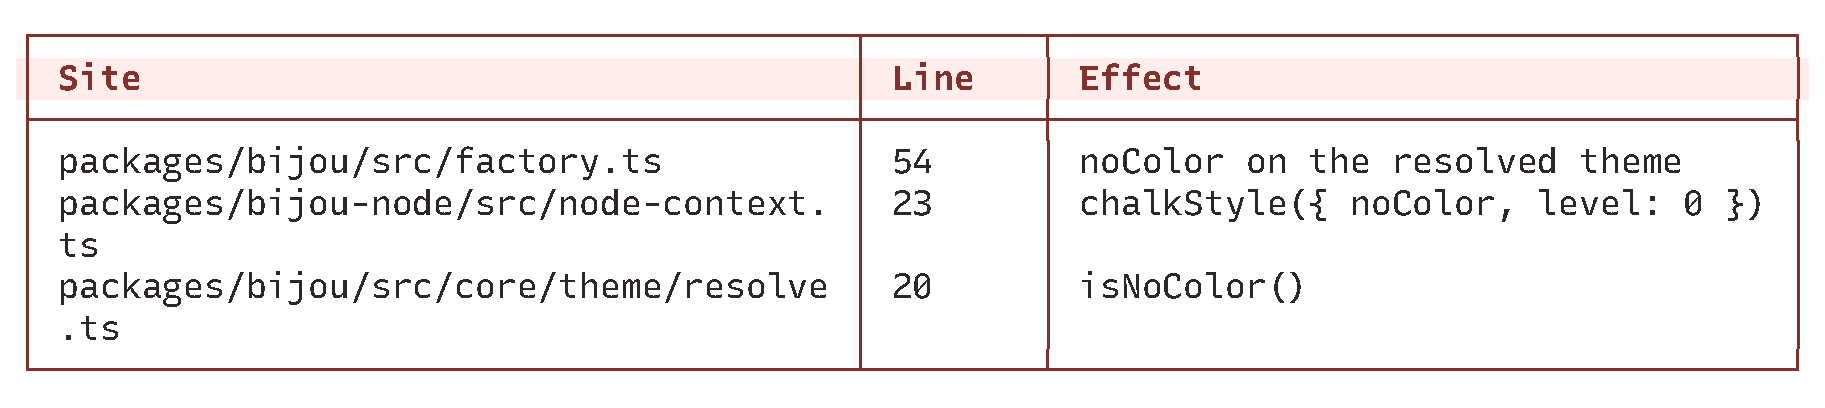
\includegraphics[width=\linewidth]{figures/tables/table-037-g1-1.pdf}
\par\smallskip{\scriptsize\color{BookMuted}Rows 1–3. Actual Bijou table component.}
\end{center}


So removing the line removes the interactivity damage while every \textbf{colour and style} escape stays suppressed. Not every escape: an interactive session by definition emits cursor movement, screen updates and possibly alternate-screen control sequences, and it should --- a monochrome TUI is still a TUI. \texttt{N\allowbreak{}O\allowbreak{}\_\allowbreak{}C\allowbreak{}O\allowbreak{}L\allowbreak{}O\allowbreak{}R} asks for no colour, not for no terminal control. The two concerns were never coupled in the implementation; only in the detector.

\texttt{g\allowbreak{}i\allowbreak{}t\allowbreak{}-\allowbreak{}c\allowbreak{}a\allowbreak{}s} (\texttt{b\allowbreak{}i\allowbreak{}n\allowbreak{}/\allowbreak{}u\allowbreak{}i\allowbreak{}/\allowbreak{}c\allowbreak{}o\allowbreak{}n\allowbreak{}t\allowbreak{}e\allowbreak{}x\allowbreak{}t\allowbreak{}.\allowbreak{}j\allowbreak{}s}) already ships a \texttt{d\allowbreak{}e\allowbreak{}t\allowbreak{}e\allowbreak{}c\allowbreak{}t\allowbreak{}C\allowbreak{}l\allowbreak{}i\allowbreak{}T\allowbreak{}u\allowbreak{}i\allowbreak{}M\allowbreak{}o\allowbreak{}d\allowbreak{}e} override for exactly this reason, with a comment saying so. When two first-party consumers independently re-implement a detector, the detector is wrong.

\subsection{2. An unknown status key renders struck through}\label{record-147-an-unknown-status-key-renders-struck-through}

\texttt{c\allowbreak{}r\allowbreak{}e\allowbreak{}a\allowbreak{}t\allowbreak{}e\allowbreak{}T\allowbreak{}h\allowbreak{}e\allowbreak{}m\allowbreak{}e\allowbreak{}A\allowbreak{}c\allowbreak{}c\allowbreak{}e\allowbreak{}s\allowbreak{}s\allowbreak{}o\allowbreak{}r\allowbreak{}s} (\texttt{p\allowbreak{}a\allowbreak{}c\allowbreak{}k\allowbreak{}a\allowbreak{}g\allowbreak{}e\allowbreak{}s\allowbreak{}/\allowbreak{}b\allowbreak{}i\allowbreak{}j\allowbreak{}o\allowbreak{}u\allowbreak{}/\allowbreak{}s\allowbreak{}r\allowbreak{}c\allowbreak{}/\allowbreak{}c\allowbreak{}o\allowbreak{}r\allowbreak{}e\allowbreak{}/\allowbreak{}t\allowbreak{}h\allowbreak{}e\allowbreak{}m\allowbreak{}e\allowbreak{}/\allowbreak{}a\allowbreak{}c\allowbreak{}c\allowbreak{}e\allowbreak{}s\allowbreak{}s\allowbreak{}o\allowbreak{}r\allowbreak{}s\allowbreak{}.\allowbreak{}t\allowbreak{}s}):

\begin{CodeBlock}
status: (key) => {
  try { return tokenGraph.get(`status.${key}`, mode); }
  catch { return tokenGraph.get('status.muted', mode); }
},
\end{CodeBlock}

\texttt{s\allowbreak{}t\allowbreak{}a\allowbreak{}t\allowbreak{}u\allowbreak{}s\allowbreak{}.\allowbreak{}m\allowbreak{}u\allowbreak{}t\allowbreak{}e\allowbreak{}d} carries \texttt{[\allowbreak{}'\allowbreak{}d\allowbreak{}i\allowbreak{}m\allowbreak{}'\allowbreak{},\allowbreak{} \allowbreak{}'\allowbreak{}s\allowbreak{}t\allowbreak{}r\allowbreak{}i\allowbreak{}k\allowbreak{}e\allowbreak{}t\allowbreak{}h\allowbreak{}r\allowbreak{}o\allowbreak{}u\allowbreak{}g\allowbreak{}h\allowbreak{}'\allowbreak{}]} in \textbf{every} shipped preset --- \texttt{b\allowbreak{}i\allowbreak{}j\allowbreak{}o\allowbreak{}u\allowbreak{}-\allowbreak{}d\allowbreak{}a\allowbreak{}r\allowbreak{}k}, \texttt{b\allowbreak{}i\allowbreak{}j\allowbreak{}o\allowbreak{}u\allowbreak{}-\allowbreak{}l\allowbreak{}i\allowbreak{}g\allowbreak{}h\allowbreak{}t}, \texttt{c\allowbreak{}y\allowbreak{}a\allowbreak{}n\allowbreak{}-\allowbreak{}m\allowbreak{}a\allowbreak{}g\allowbreak{}e\allowbreak{}n\allowbreak{}t\allowbreak{}a}, \texttt{n\allowbreak{}o\allowbreak{}r\allowbreak{}d}, \texttt{c\allowbreak{}a\allowbreak{}t\allowbreak{}p\allowbreak{}p\allowbreak{}u\allowbreak{}c\allowbreak{}c\allowbreak{}i\allowbreak{}n}, \texttt{t\allowbreak{}e\allowbreak{}a\allowbreak{}l\allowbreak{}-\allowbreak{}o\allowbreak{}r\allowbreak{}a\allowbreak{}n\allowbreak{}g\allowbreak{}e\allowbreak{}-\allowbreak{}p\allowbreak{}i\allowbreak{}n\allowbreak{}k}. That is a defensible token: ``muted'' as in retired, done, cancelled. It is the wrong thing to hand back for a key nobody defined.

\texttt{s\allowbreak{}t\allowbreak{}a\allowbreak{}t\allowbreak{}u\allowbreak{}s\allowbreak{}(\allowbreak{}k\allowbreak{}e\allowbreak{}y\allowbreak{})} takes \texttt{s\allowbreak{}t\allowbreak{}r\allowbreak{}i\allowbreak{}n\allowbreak{}g}, not a key union, so the failure is silent and total: a typo, or a key the app forgot to add to its theme, produces text with a line through it. A reader sees ``cancelled''. The app said nothing of the kind. The sibling accessor already does the right thing --- \texttt{u\allowbreak{}i\allowbreak{}(\allowbreak{})} falls back to \texttt{s\allowbreak{}e\allowbreak{}m\allowbreak{}a\allowbreak{}n\allowbreak{}t\allowbreak{}i\allowbreak{}c\allowbreak{}.\allowbreak{}p\allowbreak{}r\allowbreak{}i\allowbreak{}m\allowbreak{}a\allowbreak{}r\allowbreak{}y}, a plain token in another group --- so the fix is to make \texttt{s\allowbreak{}t\allowbreak{}a\allowbreak{}t\allowbreak{}u\allowbreak{}s\allowbreak{}(\allowbreak{})} consistent with it and fall back to \texttt{s\allowbreak{}e\allowbreak{}m\allowbreak{}a\allowbreak{}n\allowbreak{}t\allowbreak{}i\allowbreak{}c\allowbreak{}.\allowbreak{}m\allowbreak{}u\allowbreak{}t\allowbreak{}e\allowbreak{}d}, which is \texttt{d\allowbreak{}i\allowbreak{}m} and nothing else in every preset.

Found in the field: an app declared a \texttt{p\allowbreak{}a\allowbreak{}i\allowbreak{}n\allowbreak{}t\allowbreak{}.\allowbreak{}u\allowbreak{}n\allowbreak{}r\allowbreak{}e\allowbreak{}v\allowbreak{}i\allowbreak{}e\allowbreak{}w\allowbreak{}e\allowbreak{}d\allowbreak{}(\allowbreak{})} helper, dropped the matching status key from its theme as a duplicate, and shipped a painter that resolved to the strikethrough fallback. No check caught it, because no view had called it yet. \texttt{i\allowbreak{}n\allowbreak{}k\allowbreak{}S\allowbreak{}t\allowbreak{}a\allowbreak{}t\allowbreak{}u\allowbreak{}s\allowbreak{}(\allowbreak{})} in \texttt{r\allowbreak{}e\allowbreak{}s\allowbreak{}o\allowbreak{}l\allowbreak{}v\allowbreak{}e\allowbreak{}.\allowbreak{}t\allowbreak{}s} has the same fallback and the same problem.

\subsection{\texorpdfstring{3. \texttt{e\allowbreak{}x\allowbreak{}t\allowbreak{}e\allowbreak{}n\allowbreak{}d\allowbreak{}T\allowbreak{}h\allowbreak{}e\allowbreak{}m\allowbreak{}e} cannot reach \texttt{b\allowbreak{}o\allowbreak{}r\allowbreak{}d\allowbreak{}e\allowbreak{}r} or \texttt{s\allowbreak{}e\allowbreak{}m\allowbreak{}a\allowbreak{}n\allowbreak{}t\allowbreak{}i\allowbreak{}c}}{3.  cannot reach  or }}\label{record-147-extendtheme-cannot-reach-border-or-semantic}

\begin{CodeBlock}
export declare function extendTheme<S, U, G>(base: Theme, extensions: {
  status?: ...; ui?: ...; gradient?: ...; surface?: ...;
}): Theme<...>
\end{CodeBlock}

\texttt{T\allowbreak{}h\allowbreak{}e\allowbreak{}m\allowbreak{}e} has six token groups. \texttt{e\allowbreak{}x\allowbreak{}t\allowbreak{}e\allowbreak{}n\allowbreak{}d\allowbreak{}T\allowbreak{}h\allowbreak{}e\allowbreak{}m\allowbreak{}e} can extend four. There is no way to override a border or semantic token through it, which matters because the shipped themes alias heavily across groups: \texttt{b\allowbreak{}i\allowbreak{}j\allowbreak{}o\allowbreak{}u\allowbreak{}-\allowbreak{}d\allowbreak{}a\allowbreak{}r\allowbreak{}k} uses \texttt{\#\allowbreak{}f\allowbreak{}2\allowbreak{}c\allowbreak{}4\allowbreak{}5\allowbreak{}d} for \texttt{s\allowbreak{}t\allowbreak{}a\allowbreak{}t\allowbreak{}u\allowbreak{}s\allowbreak{}.\allowbreak{}w\allowbreak{}a\allowbreak{}r\allowbreak{}n\allowbreak{}i\allowbreak{}n\allowbreak{}g}, \texttt{s\allowbreak{}t\allowbreak{}a\allowbreak{}t\allowbreak{}u\allowbreak{}s\allowbreak{}.\allowbreak{}a\allowbreak{}c\allowbreak{}t\allowbreak{}i\allowbreak{}v\allowbreak{}e}, \texttt{s\allowbreak{}e\allowbreak{}m\allowbreak{}a\allowbreak{}n\allowbreak{}t\allowbreak{}i\allowbreak{}c\allowbreak{}.\allowbreak{}w\allowbreak{}a\allowbreak{}r\allowbreak{}n\allowbreak{}i\allowbreak{}n\allowbreak{}g}, \texttt{s\allowbreak{}e\allowbreak{}m\allowbreak{}a\allowbreak{}n\allowbreak{}t\allowbreak{}i\allowbreak{}c\allowbreak{}.\allowbreak{}a\allowbreak{}c\allowbreak{}c\allowbreak{}e\allowbreak{}n\allowbreak{}t}, \texttt{u\allowbreak{}i\allowbreak{}.\allowbreak{}c\allowbreak{}u\allowbreak{}r\allowbreak{}s\allowbreak{}o\allowbreak{}r}, \texttt{u\allowbreak{}i\allowbreak{}.\allowbreak{}f\allowbreak{}o\allowbreak{}c\allowbreak{}u\allowbreak{}s\allowbreak{}G\allowbreak{}u\allowbreak{}t\allowbreak{}t\allowbreak{}e\allowbreak{}r}, \texttt{u\allowbreak{}i\allowbreak{}.\allowbreak{}s\allowbreak{}e\allowbreak{}c\allowbreak{}t\allowbreak{}i\allowbreak{}o\allowbreak{}n\allowbreak{}H\allowbreak{}e\allowbreak{}a\allowbreak{}d\allowbreak{}e\allowbreak{}r}, \texttt{u\allowbreak{}i\allowbreak{}.\allowbreak{}l\allowbreak{}o\allowbreak{}g\allowbreak{}o}, \texttt{b\allowbreak{}o\allowbreak{}r\allowbreak{}d\allowbreak{}e\allowbreak{}r\allowbreak{}.\allowbreak{}s\allowbreak{}e\allowbreak{}c\allowbreak{}o\allowbreak{}n\allowbreak{}d\allowbreak{}a\allowbreak{}r\allowbreak{}y} \textbf{and} \texttt{b\allowbreak{}o\allowbreak{}r\allowbreak{}d\allowbreak{}e\allowbreak{}r\allowbreak{}.\allowbreak{}w\allowbreak{}a\allowbreak{}r\allowbreak{}n\allowbreak{}i\allowbreak{}n\allowbreak{}g} --- ten aliases of one amber.

An app that calls \texttt{e\allowbreak{}x\allowbreak{}t\allowbreak{}e\allowbreak{}n\allowbreak{}d\allowbreak{}T\allowbreak{}h\allowbreak{}e\allowbreak{}m\allowbreak{}e\allowbreak{}(\allowbreak{}B\allowbreak{}I\allowbreak{}J\allowbreak{}O\allowbreak{}U\allowbreak{}\_\allowbreak{}D\allowbreak{}A\allowbreak{}R\allowbreak{}K\allowbreak{},\allowbreak{} \allowbreak{}\{\allowbreak{} \allowbreak{}s\allowbreak{}t\allowbreak{}a\allowbreak{}t\allowbreak{}u\allowbreak{}s\allowbreak{} \allowbreak{}\}\allowbreak{})} therefore replaces its statuses and silently keeps bijou's amber for every heading, cursor and border. In the case that prompted this, the app's section headings landed ΔE \textbf{0.023} from its own \texttt{w\allowbreak{}a\allowbreak{}r\allowbreak{}n\allowbreak{}i\allowbreak{}n\allowbreak{}g} in OKLab --- indistinguishable --- and the only escape was to abandon \texttt{e\allowbreak{}x\allowbreak{}t\allowbreak{}e\allowbreak{}n\allowbreak{}d\allowbreak{}T\allowbreak{}h\allowbreak{}e\allowbreak{}m\allowbreak{}e} and author all six groups by hand.

\section{Non-goals}\label{record-147-non-goals}

\begin{itemize}
\tightlist
\item
  \textbf{Changing \texttt{s\allowbreak{}t\allowbreak{}a\allowbreak{}t\allowbreak{}u\allowbreak{}s\allowbreak{}.\allowbreak{}m\allowbreak{}u\allowbreak{}t\allowbreak{}e\allowbreak{}d} itself.} Its strikethrough is deliberate and used. Only the \emph{fallback target} moves.
\item
  \textbf{Re-fitting the shipped palettes.} The \texttt{\#\allowbreak{}f\allowbreak{}2\allowbreak{}c\allowbreak{}4\allowbreak{}5\allowbreak{}d} ten-way alias and \texttt{b\allowbreak{}i\allowbreak{}j\allowbreak{}o\allowbreak{}u\allowbreak{}-\allowbreak{}d\allowbreak{}a\allowbreak{}r\allowbreak{}k}'s error/success collapse under protanopia (ΔE 0.059) are real, are what motivated non-goal-adjacent issues, and are filed separately.
\item
  \textbf{Adding OKLCH authoring or a CVD-aware palette audit to bijou.} Also filed separately; \texttt{d\allowbreak{}o\allowbreak{}c\allowbreak{}t\allowbreak{}o\allowbreak{}r\allowbreak{}T\allowbreak{}h\allowbreak{}e\allowbreak{}m\allowbreak{}e} covers contrast and reuse but not perceptual separation under simulated colour-vision deficiency.
\item
  \textbf{Typing \texttt{s\allowbreak{}t\allowbreak{}a\allowbreak{}t\allowbreak{}u\allowbreak{}s\allowbreak{}(\allowbreak{}k\allowbreak{}e\allowbreak{}y\allowbreak{})} to a key union.} It would catch defect 2 at compile time for typed callers, but it is a wider API change than this cycle wants and would not help JS consumers. Filed as follow-up.
\end{itemize}

\section{Playback questions}\label{record-147-playback-questions}

\begin{enumerate}
\def\labelenumi{\arabic{enumi}.}
\tightlist
\item
  With \texttt{N\allowbreak{}O\allowbreak{}\_\allowbreak{}C\allowbreak{}O\allowbreak{}L\allowbreak{}O\allowbreak{}R\allowbreak{}=\allowbreak{}1} and a real TTY on both stdio, is \texttt{c\allowbreak{}t\allowbreak{}x\allowbreak{}.\allowbreak{}m\allowbreak{}o\allowbreak{}d\allowbreak{}e} \texttt{'\allowbreak{}i\allowbreak{}n\allowbreak{}t\allowbreak{}e\allowbreak{}r\allowbreak{}a\allowbreak{}c\allowbreak{}t\allowbreak{}i\allowbreak{}v\allowbreak{}e\allowbreak{}'}?
\item
  With \texttt{N\allowbreak{}O\allowbreak{}\_\allowbreak{}C\allowbreak{}O\allowbreak{}L\allowbreak{}O\allowbreak{}R\allowbreak{}=\allowbreak{}1}, is \texttt{t\allowbreak{}h\allowbreak{}e\allowbreak{}m\allowbreak{}e\allowbreak{}.\allowbreak{}n\allowbreak{}o\allowbreak{}C\allowbreak{}o\allowbreak{}l\allowbreak{}o\allowbreak{}r} still \texttt{t\allowbreak{}r\allowbreak{}u\allowbreak{}e} and does \texttt{s\allowbreak{}t\allowbreak{}y\allowbreak{}l\allowbreak{}e\allowbreak{}d\allowbreak{}(\allowbreak{})} still return unstyled text? And with \texttt{N\allowbreak{}O\allowbreak{}\_\allowbreak{}C\allowbreak{}O\allowbreak{}L\allowbreak{}O\allowbreak{}R\allowbreak{}=\allowbreak{}"\allowbreak{}"} --- the variable is presence-only, so an implementation that special-cases \texttt{'\allowbreak{}1\allowbreak{}'} must not pass.
\item
  Does \texttt{T\allowbreak{}E\allowbreak{}R\allowbreak{}M\allowbreak{}=\allowbreak{}d\allowbreak{}u\allowbreak{}m\allowbreak{}b} still yield \texttt{'\allowbreak{}p\allowbreak{}i\allowbreak{}p\allowbreak{}e\allowbreak{}'}? Does a non-TTY stdout? Does \texttt{C\allowbreak{}I} still yield \texttt{'\allowbreak{}s\allowbreak{}t\allowbreak{}a\allowbreak{}t\allowbreak{}i\allowbreak{}c\allowbreak{}'}, and \texttt{B\allowbreak{}I\allowbreak{}J\allowbreak{}O\allowbreak{}U\allowbreak{}\_\allowbreak{}A\allowbreak{}C\allowbreak{}C\allowbreak{}E\allowbreak{}S\allowbreak{}S\allowbreak{}I\allowbreak{}B\allowbreak{}L\allowbreak{}E\allowbreak{}=\allowbreak{}1} still win outright?
\item
  Does \texttt{s\allowbreak{}t\allowbreak{}a\allowbreak{}t\allowbreak{}u\allowbreak{}s\allowbreak{}(\allowbreak{}'\allowbreak{}n\allowbreak{}o\allowbreak{}n\allowbreak{}e\allowbreak{}x\allowbreak{}i\allowbreak{}s\allowbreak{}t\allowbreak{}e\allowbreak{}n\allowbreak{}t\allowbreak{}'\allowbreak{})} return a token with no \texttt{s\allowbreak{}t\allowbreak{}r\allowbreak{}i\allowbreak{}k\allowbreak{}e\allowbreak{}t\allowbreak{}h\allowbreak{}r\allowbreak{}o\allowbreak{}u\allowbreak{}g\allowbreak{}h}?
\item
  Does \texttt{s\allowbreak{}t\allowbreak{}a\allowbreak{}t\allowbreak{}u\allowbreak{}s\allowbreak{}(\allowbreak{}'\allowbreak{}m\allowbreak{}u\allowbreak{}t\allowbreak{}e\allowbreak{}d\allowbreak{}'\allowbreak{})} still return the real muted token, strikethrough intact?
\item
  Does \texttt{i\allowbreak{}n\allowbreak{}k\allowbreak{}S\allowbreak{}t\allowbreak{}a\allowbreak{}t\allowbreak{}u\allowbreak{}s\allowbreak{}(\allowbreak{}'\allowbreak{}n\allowbreak{}o\allowbreak{}n\allowbreak{}e\allowbreak{}x\allowbreak{}i\allowbreak{}s\allowbreak{}t\allowbreak{}e\allowbreak{}n\allowbreak{}t\allowbreak{}'\allowbreak{})} agree with \texttt{s\allowbreak{}t\allowbreak{}a\allowbreak{}t\allowbreak{}u\allowbreak{}s\allowbreak{}(\allowbreak{})} about the fallback?
\item
  Does \texttt{e\allowbreak{}x\allowbreak{}t\allowbreak{}e\allowbreak{}n\allowbreak{}d\allowbreak{}T\allowbreak{}h\allowbreak{}e\allowbreak{}m\allowbreak{}e\allowbreak{}(\allowbreak{}b\allowbreak{}a\allowbreak{}s\allowbreak{}e\allowbreak{},\allowbreak{} \allowbreak{}\{\allowbreak{} \allowbreak{}b\allowbreak{}o\allowbreak{}r\allowbreak{}d\allowbreak{}e\allowbreak{}r\allowbreak{},\allowbreak{} \allowbreak{}s\allowbreak{}e\allowbreak{}m\allowbreak{}a\allowbreak{}n\allowbreak{}t\allowbreak{}i\allowbreak{}c\allowbreak{} \allowbreak{}\}\allowbreak{})} merge those groups, preserve unlisted keys within them, and leave the other four groups untouched?
\end{enumerate}

\section{Decision}\label{record-147-decision}

\begin{enumerate}
\def\labelenumi{\arabic{enumi}.}
\tightlist
\item
  Delete the \texttt{N\allowbreak{}O\allowbreak{}\_\allowbreak{}C\allowbreak{}O\allowbreak{}L\allowbreak{}O\allowbreak{}R} branch from \texttt{d\allowbreak{}e\allowbreak{}t\allowbreak{}e\allowbreak{}c\allowbreak{}t\allowbreak{}O\allowbreak{}u\allowbreak{}t\allowbreak{}p\allowbreak{}u\allowbreak{}t\allowbreak{}M\allowbreak{}o\allowbreak{}d\allowbreak{}e}. Update its docblock and the \texttt{O\allowbreak{}u\allowbreak{}t\allowbreak{}p\allowbreak{}u\allowbreak{}t\allowbreak{}M\allowbreak{}o\allowbreak{}d\allowbreak{}e} doc comment, which both currently document the old order.
\item
  Point the \texttt{s\allowbreak{}t\allowbreak{}a\allowbreak{}t\allowbreak{}u\allowbreak{}s\allowbreak{}(\allowbreak{})} accessor and \texttt{i\allowbreak{}n\allowbreak{}k\allowbreak{}S\allowbreak{}t\allowbreak{}a\allowbreak{}t\allowbreak{}u\allowbreak{}s\allowbreak{}(\allowbreak{})} fallbacks at \texttt{s\allowbreak{}e\allowbreak{}m\allowbreak{}a\allowbreak{}n\allowbreak{}t\allowbreak{}i\allowbreak{}c\allowbreak{}.\allowbreak{}m\allowbreak{}u\allowbreak{}t\allowbreak{}e\allowbreak{}d}.
\item
  Add optional \texttt{b\allowbreak{}o\allowbreak{}r\allowbreak{}d\allowbreak{}e\allowbreak{}r} and \texttt{s\allowbreak{}e\allowbreak{}m\allowbreak{}a\allowbreak{}n\allowbreak{}t\allowbreak{}i\allowbreak{}c} to \texttt{e\allowbreak{}x\allowbreak{}t\allowbreak{}e\allowbreak{}n\allowbreak{}d\allowbreak{}T\allowbreak{}h\allowbreak{}e\allowbreak{}m\allowbreak{}e}'s extension parameter.
\end{enumerate}

\section{Breaking-change note}\label{record-147-breaking-change-note}

1 and 2 change observable behaviour that the current docblocks describe, so this lands as part of \textbf{8.0.0} rather than a minor.

\textbf{Eight existing tests across five files} assert the behaviour being removed. Six of them encode the \texttt{N\allowbreak{}O\allowbreak{}\_\allowbreak{}C\allowbreak{}O\allowbreak{}L\allowbreak{}O\allowbreak{}R} → \texttt{'\allowbreak{}p\allowbreak{}i\allowbreak{}p\allowbreak{}e\allowbreak{}'} mapping alone:

\begin{center}
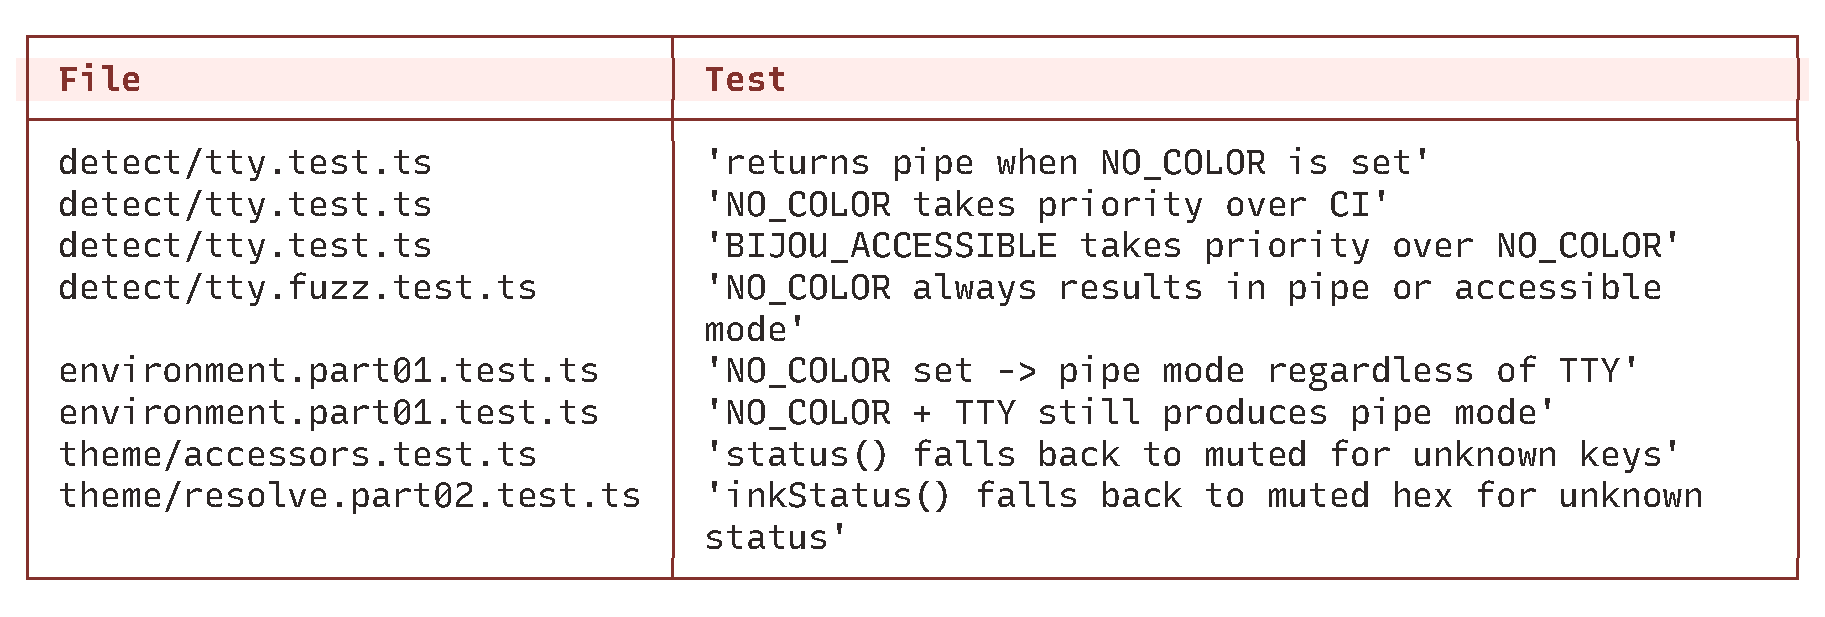
\includegraphics[width=\linewidth]{figures/tables/table-038-g1-1.pdf}
\par\smallskip{\scriptsize\color{BookMuted}Rows 1–8. Actual Bijou table component.}
\end{center}


Six tests reinforcing a rule usually means the rule was chosen deliberately. It was not. Every one is a characterization test restating the truth table, sitting in \texttt{d\allowbreak{}e\allowbreak{}s\allowbreak{}c\allowbreak{}r\allowbreak{}i\allowbreak{}b\allowbreak{}e} blocks named ``detection logic'' and ``conflicting env vars'', and no comment, docblock, or design note in the repository argues \emph{why} \texttt{N\allowbreak{}O\allowbreak{}\_\allowbreak{}C\allowbreak{}O\allowbreak{}L\allowbreak{}O\allowbreak{}R} should imply non-interactive --- the only justification is the detector's own docblock restating its own order. The tests are thorough about coverage, not about defending the choice.

They are not wrong about what the code did; they are the specification of the defect. They are rewritten to assert the new contract, and this section exists so that the rewrite is a recorded decision rather than tests quietly edited to make a build go green. Two of them change shape rather than expectation:

\begin{itemize}
\tightlist
\item
  \texttt{'\allowbreak{}B\allowbreak{}I\allowbreak{}J\allowbreak{}O\allowbreak{}U\allowbreak{}\_\allowbreak{}A\allowbreak{}C\allowbreak{}C\allowbreak{}E\allowbreak{}S\allowbreak{}S\allowbreak{}I\allowbreak{}B\allowbreak{}L\allowbreak{}E\allowbreak{} \allowbreak{}t\allowbreak{}a\allowbreak{}k\allowbreak{}e\allowbreak{}s\allowbreak{} \allowbreak{}p\allowbreak{}r\allowbreak{}i\allowbreak{}o\allowbreak{}r\allowbreak{}i\allowbreak{}t\allowbreak{}y\allowbreak{} \allowbreak{}o\allowbreak{}v\allowbreak{}e\allowbreak{}r\allowbreak{} \allowbreak{}N\allowbreak{}O\allowbreak{}\_\allowbreak{}C\allowbreak{}O\allowbreak{}L\allowbreak{}O\allowbreak{}R\allowbreak{}'} becomes vacuous once \texttt{N\allowbreak{}O\allowbreak{}\_\allowbreak{}C\allowbreak{}O\allowbreak{}L\allowbreak{}O\allowbreak{}R} no longer affects mode, and is reframed as priority over an interactive TTY.
\item
  the fuzz property is strengthened rather than adjusted. Instead of asserting which mode results, it now asserts that adding \texttt{N\allowbreak{}O\allowbreak{}\_\allowbreak{}C\allowbreak{}O\allowbreak{}L\allowbreak{}O\allowbreak{}R} to \emph{any} environment leaves that environment's mode unchanged --- the contract stated directly.
\end{itemize}

\texttt{r\allowbreak{}e\allowbreak{}s\allowbreak{}o\allowbreak{}l\allowbreak{}v\allowbreak{}e\allowbreak{}.\allowbreak{}p\allowbreak{}a\allowbreak{}r\allowbreak{}t\allowbreak{}0\allowbreak{}2\allowbreak{}.\allowbreak{}t\allowbreak{}e\allowbreak{}s\allowbreak{}t\allowbreak{}.\allowbreak{}t\allowbreak{}s} is the one case with no observable behaviour change: \texttt{i\allowbreak{}n\allowbreak{}k\allowbreak{}S\allowbreak{}t\allowbreak{}a\allowbreak{}t\allowbreak{}u\allowbreak{}s\allowbreak{}(\allowbreak{})} returns a hex, and \texttt{s\allowbreak{}t\allowbreak{}a\allowbreak{}t\allowbreak{}u\allowbreak{}s\allowbreak{}.\allowbreak{}m\allowbreak{}u\allowbreak{}t\allowbreak{}e\allowbreak{}d} and \texttt{s\allowbreak{}e\allowbreak{}m\allowbreak{}a\allowbreak{}n\allowbreak{}t\allowbreak{}i\allowbreak{}c\allowbreak{}.\allowbreak{}m\allowbreak{}u\allowbreak{}t\allowbreak{}e\allowbreak{}d} share a hex in every shipped preset. It is updated anyway so the two fallbacks cannot disagree in a theme where the hexes differ.

3 is additive and breaks nothing.

\section{Acceptance criteria}\label{record-147-acceptance-criteria}

\begin{itemize}
\tightlist
\item
  All seven playback questions have a passing test.
\item
  \texttt{n\allowbreak{}p\allowbreak{}m\allowbreak{} \allowbreak{}r\allowbreak{}u\allowbreak{}n\allowbreak{} \allowbreak{}l\allowbreak{}i\allowbreak{}n\allowbreak{}t}, the full test suite, and the Code Dojo gates pass.
\item
  \texttt{d\allowbreak{}o\allowbreak{}c\allowbreak{}s\allowbreak{}/\allowbreak{}C\allowbreak{}H\allowbreak{}A\allowbreak{}N\allowbreak{}G\allowbreak{}E\allowbreak{}L\allowbreak{}O\allowbreak{}G\allowbreak{}.\allowbreak{}m\allowbreak{}d} records all three under a \texttt{C\allowbreak{}h\allowbreak{}a\allowbreak{}n\allowbreak{}g\allowbreak{}e\allowbreak{}d} heading with the breaking note, and \texttt{d\allowbreak{}o\allowbreak{}c\allowbreak{}s\allowbreak{}/\allowbreak{}B\allowbreak{}E\allowbreak{}A\allowbreak{}R\allowbreak{}I\allowbreak{}N\allowbreak{}G\allowbreak{}.\allowbreak{}m\allowbreak{}d} mentions the detection-semantics change.
\item
  No consumer-visible colour output changes when \texttt{N\allowbreak{}O\allowbreak{}\_\allowbreak{}C\allowbreak{}O\allowbreak{}L\allowbreak{}O\allowbreak{}R} is set.
\end{itemize}

